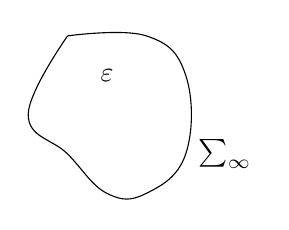
\begin{tikzpicture}

\draw  plot[smooth, tension=.7] coordinates {(0.5,0.5) (0,-0.5) (0.5,-1) (1,-1.5) (1.5,-1.5) (2,-1) (2,0) (1.5,0.5) (0.5,0.5)};
\node at (1,0) {$\varepsilon$};
\node at (2.5,-1) {$\sum_\infty$};
\end{tikzpicture}